	\chapter{Kravspecifikation}
	
	\section{Systembeskrivelse}
	Systemet består af en database med brugeradgang via iOS applikation.
	Databasen indeholder brugere, projekter, PDF tegninger og data om projekterne.
	Et projekt indeholder en PDF tegning, tegne objekter, mulighed for upload af billede og tekst.
	
	\begin{figure}[H]
		\centering
		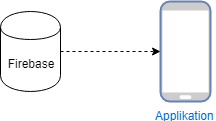
\includegraphics[width=0.4\linewidth]{Kravspecifikation/Oversigtoversystem}
		\caption{Oversigt over systemet}
		\label{fig:OversigtSystembeskrivelse}
	\end{figure}
	
	Systemet skal kunne håndtere de bygge projekter Rambøll har, og oprette nye når de overtager et nyt bygge projekt.
	Disse skal kunne tilgåes af Rambøll ansatte, via enten en smartphone eller tablet.
	Rambøll ansatte får tildelt et personligt login.
	Brugere skal kunne oprette en registring for et givet projekt.
	Når en bruger er færdig med at oprette sin registrering, skal denne kunne exportes til en excel fil og sendes som en vedhæftet fil i en mail.
	Systemet har en log, som indeholder en liste over alle registreringer, til et givent projekt. \\	
			
	\section{Afgrænsning}
	SOME TEXT
	
	\clearpage
		

\section{User stories} \label{sec:UserStories}
Følgende er en beskrivelse af de aktuelle krav stillet til projektet. De er alle opstillet som user stories. User stories er korte beskrivelser af funktionalitet, som står på en fast form. De er let læselige og har værdi for både personer direkte involveret i projektet og udefrakommende, som skal opnå en idé om kravene til projektet. 

\subsection{Aktør kontekst diagram}\label{sec:aktor}
	På figur \ref{fig:AktorKontekst} ses aktør kontekst diagrammet for Rambøll Tilsyn. Diagrammet viser hvilke aktør der interagere med systemet.
\begin{figure}[H]
	\centering
	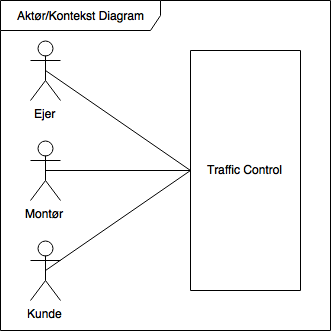
\includegraphics[width=0.5\linewidth]{Kravspecifikation/AktorDiagram}
	\caption{Aktør kontekst diagram for Rambøll Tilsyn}
	\label{fig:AktorKontekst}
\end{figure}


\subsection{User stories beskrevet med Gherkin}
Til beskrivelse af user stories er Gherkin-syntaksen valgt, hvor stories 
kan skrives på et flydende sprog, mens de er testbare.\cite{Gherkin} Dette kaldes også et Business-Readable Domain  
Specific Language. En særlig fordel ved anvendelsen af syntaksen er at den er opstiller kravene så de er særligt testbare, hvilket medfører at kravene for test af features er skrevet i user stories.
Gherkin anvender nøgleord (i det flg. afsnit 
markeret med blåt), som hver især har en funktion i beskrivelsen af hver 
user story.  \vspace{0.2 cm}\\
Første del af en egenskab indeholder en beskrivelse af forretningsdomænet. 
Formatet i	dette afsnit vælges frit. Det anbefales, at man anvender et 
system, hvor der som minimum svares på hvilke aktører der har et behov, hvad 
behovet består af og hvorfor aktører har dette behov. En tre trins user 
story opfylder dette krav og opstilles med tre 
sætninger. Første sætning svarer på hvilken aktør, eller aktører der har
behovet. Dernæst svarer man på hvad det konkret er at aktøreren ønsker at 
opnå. Den tredje sætning beskriver aktørens motivation for at anvende 
funktionaliteten\\
Samtlige nøgleord beskrives nedenfor:

\large{\textbf{Givet}}\\
Disse trin definerer tilstande og datastrukturer som anvendes i de 
efterfølgende trin og scenarier.\\
\large{\textbf{Når}}\\
Disse trin beskriver handlinger som ændrer Scenariets tilstand. Dette kan 
være handlinger	foretaget af aktøreren og/eller systemet.\\
\large{\textbf{Så}}\\
Disse trin definerer udfaldet af forudgående handlinger i et givet 
scenarie. Alle scenarier skal afsluttes ved at definere et det forventede 
udfald i et eller flere "Så"trin.\\

\clearpage

\large{\textbf{Scenarier}}\\
Scenarier er samlinger af trin som definerer de funktionelle krav til 
forløb. Første scenarie i en egenskab dækker hovedfunktionaliteten. De 
efterfølgende scenarier dækker fejlhåndteringer og alternative scenarier.\\
\large{\textbf{Baggrund}}\\
Baggrund er en særlig type scenarie som udføres inden hvert af de 
efterfølgende scenarier	i egenskaben. Systemets tilstand og preconditions 
beskrives under overskriften "Baggrund" efterfulgt af et kolon og 
linjeskift. Herefter listes alle de data, tilstande og handlinger som udgør 
systemets tilstand inden samtlige af de efterfølgende Scenarier kan	udføres.


\subsubsection{Log ind}
\textbf{\textsc{\textcolor{RoyalBlue} {Egenskab:} Log-in på applikationen}} \\
Som bruger\\
Ønsker jeg at kunne logge ind på applikationen\\
For at kunne benytte applikationen\\

\textbf{\textsc{\color{RoyalBlue}Baggrund:}}\\
\textcolor{RoyalBlue}{Givet} følgende eksisterende profil\\
\begin{tabular}{| l | l | l | l |}
	\textbf{fornavn} & \textbf{efternavn} & \textbf{e-mail} & \textbf{kode} \\
	Ao & Testbruger & Ao@mail.dk & letmein\\
\end{tabular}
\newline \newline
\textcolor{RoyalBlue}{Og} "Ao" er ikke allerede logget ind i systemet\\
\textcolor{RoyalBlue}{Og} han har navigeret til applikationens log-in side\\

\textbf{\textsc{\textcolor{RoyalBlue}{Scenarie:}} Log ind med korrekte oplysninger}\\
\textcolor{RoyalBlue}{Når} "Ao" indtaster sin mail og kode i de korrekte tekstfelter\\
\textcolor{RoyalBlue}{Og} han trykker på log-in knappen\\
\textcolor{RoyalBlue}{Så} navigeres han til applikationens forside\\

\textbf{\textsc{\textcolor{RoyalBlue}{Scenarie:}} Log ind med forkerte oplysninger} \\
\textcolor{RoyalBlue}{Når} "Ao" indtaster følgende oplysninger:\\
\begin{tabular}{| l | l |}
	\textbf{e-mail} & \textbf{kode}\\
	Ao@mail.dk & 123\\
\end{tabular}
\newline \newline
\textcolor{RoyalBlue}{Og} han trykker på log-in knappen\\
\textcolor{RoyalBlue}{Så} informeres han om, at der er indtastet forkerte oplysninger\\
\textcolor{RoyalBlue}{Og} han bliver på log-in siden\\

\clearpage

\subsubsection{Opret bruger} \label{sec:USOpretBruger}
\textbf{\textsc{\textcolor{RoyalBlue}{Egenskab:} Opret bruger}} \\
Som bruger\\
Ønsker jeg at kunne oprette en bruger på applikationen\\
For at kunne give en anden bruger adgang til systemet\\

\textcolor{RoyalBlue}{\textbf{\textsc{Baggrund:}}}\\
\textcolor{RoyalBlue}{Givet} at brugeren "Rasmus" er logget ind \\
\textcolor{RoyalBlue}{Og} han vil oprette en bruger med følgende oplysninger:\\
\begin{tabular}{| l | l |}
	\textbf{e-mail} & \textbf{kode} \\
	morten@ramboell.dk & solskin\\
\end{tabular}
\newline \newline
\textcolor{RoyalBlue}{Og} han er navigeret til opret bruger siden for at oprette brugere\\

\textbf{\textsc{\textcolor{RoyalBlue}{Scenarie:}} Opret bruger}\\
\textcolor{RoyalBlue}{Når} "Rasmus" indtaster mail, kode, telefonnummer, 
fornavn og efternavn \\
\textcolor{RoyalBlue}{Og} trykker på opret bruger-knappen\\
\textcolor{RoyalBlue}{Så} oprettes den nye bruger\\
\textcolor{RoyalBlue}{Og} den nye bruger kan logge ind\\


\subsubsection{Ændring af brugeroplysninger}
\textbf{\textsc{\textcolor{RoyalBlue}{Egenskab:} Ændring af brugeroplysninger}}\\
Som bruger\\
Ønsker jeg at kunne ændre brugeroplysninger\\
For at have aktuelle oplysninger\\

\textsc{\textcolor{RoyalBlue}{\textbf{Baggrund:}}}\\
\textcolor{RoyalBlue}{Givet} at "Niels" er logget ind\\
\textcolor{RoyalBlue}{Og} han har følgende nuværende oplysninger:\\
\begin{tabular}{| l | l | l |}
	\textbf{fornavn} & \textbf{efternavn} & \textbf{kodeord} \\
	Niels & Testbruger & paris \\
\end{tabular}
\newline \newline
\textcolor{RoyalBlue}{Og} at hun vil ændre indstillingerne til følgende:\\
\begin{tabular}{| l | l | l | l |}
	\textbf{fornavn} & \textbf{efternavn} & \textbf{kodeord} \\
	Cille & TestTest & london \\
\end{tabular}
\newline \newline
\textcolor{RoyalBlue}{Og} at han er navigeret til rediger bruger siden\\

\textbf{\textsc{\textcolor{RoyalBlue}{Scenarie:}} Ændr kode}\\-
\textcolor{RoyalBlue}{Når} "Niels" indtaster "paris" i kodefeltet "Gammel adgangskode"\\
\textcolor{RoyalBlue}{Og} han skriver "london" i "Ny adgangskode" og "Bekræft ny adgangskode"\\
\textcolor{RoyalBlue}{Og} han trykker på gem oplysninger\\
\textcolor{RoyalBlue}{Så} gemmes oplysningerne\\
\textcolor{RoyalBlue}{Og} han informeres om at ændringerne er gemt\\

\textbf{\textsc{\textcolor{RoyalBlue}{Scenarie:}} Ændr for- og efternavn}\\
\textcolor{RoyalBlue}{Når} "Niels" indtaster nyt for- og efternavn i de korrekte tekstfelter\\
\textcolor{RoyalBlue}{Og} han trykker på ok\\
\textcolor{RoyalBlue}{Så} gemmes oplysningerne\\
\textcolor{RoyalBlue}{Og} han kan se at ændringerne er gemt\\

\textbf{\textsc{\textcolor{RoyalBlue}{Scenarie:}} Ændr telefonnummer}\\
\textcolor{RoyalBlue}{Når} "Niels" indtaster "87654321" i det korrekte tekstfelt\\
\textcolor{RoyalBlue}{Og} han trykker på ok\\
\textcolor{RoyalBlue}{Så} gemmes oplysningerne\\
\textcolor{RoyalBlue}{Og} han kan se at ændringerne er gemt\\

\subsubsection{Opret en registrering på PDF tegning} %\label{sec:USOpretSag}
\textbf{\textsc{\textcolor{RoyalBlue}{Egenskab:} Opret en registrering på PDF tegning}}\\
Som bruger\\
Ønsker jeg at kunne oprette en registrering på en PDF\\
For kunne lave en registrering på et givent projekts pdf tegning\\

\textsc{\textcolor{RoyalBlue}{\textbf{Baggrund:}}}\\
\textcolor{RoyalBlue}{Givet} at "Søren" er logget ind\\
\textcolor{RoyalBlue}{Og} han har følgende nuværende oplysninger:\\
\begin{tabular}{| l | l |}
	\textbf{fornavn} & \textbf{rolle} \\
	Søren & Bruger\\
\end{tabular}

\textbf{\textsc{\textcolor{RoyalBlue}{Scenarie:}} Opret en registrering på PDF tegning}\\
\textcolor{RoyalBlue}{Når} Søren vælger "Opret registrering på PDF tegning"\\
\textcolor{RoyalBlue}{Så}  navigeres han videre til registrerings siden\\
\textcolor{RoyalBlue}{Så}  har han mulighed for at indsætte objekter på PDF'en som en del af hans registrering\\
\textcolor{RoyalBlue}{Når} han er færdig med at registrer kan han vælge afslut \\
\textcolor{RoyalBlue}{Så}  navigeres hans videre til fejl rapporten for alle objekter oprettet på projektet \\

\subsubsection{Opret fluebens opbjekt på PDF tegning} %\label{sec:USOpretSag}
\textbf{\textsc{\textcolor{RoyalBlue}{Egenskab:} Opret fluebens opbjekt på PDF tegning}}\\
Som bruger\\
Ønsker jeg at kunne oprette et fluebens objekt på en PDF\\
For kunne redigere min registrering på et givent projekts pdf tegning\\

\textsc{\textcolor{RoyalBlue}{\textbf{Baggrund:}}}\\
\textcolor{RoyalBlue}{Givet} at "Søren" er logget ind\\
\textcolor{RoyalBlue}{Og} han har følgende nuværende oplysninger:\\
\begin{tabular}{| l | l |}
	\textbf{fornavn} & \textbf{rolle} \\
	Søren & Bruger\\
\end{tabular}

!!!!!!!!!!!!!!!!!!

\textbf{\textsc{\textcolor{RoyalBlue}{Scenarie:}} Opret fluebens opbjekt på PDF tegning}\\
\textcolor{RoyalBlue}{Når} Søren vælger "Opret registrering på PDF tegning"\\
\textcolor{RoyalBlue}{Så}  navigeres han videre til registrerings siden\\
\textcolor{RoyalBlue}{Så}  har han mulighed for at indsætte objekter på PDF'en som en del af hans registrering\\
\textcolor{RoyalBlue}{Når} han er færdig med at registrer kan han vælge afslut \\
\textcolor{RoyalBlue}{Så}  navigeres hans videre til fejl rapporten for alle objekter oprettet på projektet \\

\subsubsection{Opret en registrering uden PDF tegning}
\textbf{\textsc{\textcolor{RoyalBlue}{Egenskab:} Opret en registrering uden PDF tegning}}\\
Som bruger\\
Ønsker jeg at kunne oprette en registrering uden en PDF\\
For kunne lave en registrering på et givent projekt\\

\textsc{\textcolor{RoyalBlue}{\textbf{Baggrund:}}}\\
\textcolor{RoyalBlue}{Givet} at "Dan" er logget ind\\
\textcolor{RoyalBlue}{Og} han har følgende nuværende oplysninger:\\
\begin{tabular}{| l | l |}
	\textbf{fornavn} & \textbf{rolle} \\
	Dan & Bruger\\
\end{tabular}
\newline \newline

\textbf{\textsc{\textcolor{RoyalBlue}{Scenarie:}} Opret en registrering uden PDF tegning}\\
\textcolor{RoyalBlue}{Når} Dan vælger "Opret registrering uden PDF tegning"\\
\textcolor{RoyalBlue}{Så} navigeres han videre til registrerings siden\\
\textcolor{RoyalBlue}{Så} har han mulighed for at indsætte billede objekter på den tomme PDF\\
\textcolor{RoyalBlue}{Når} an er færdig med at registrer kan han vælge afslut\\
\textcolor{RoyalBlue}{Så} navigeres hans videre til tilsyns rapporten for hans registrering\\

\subsubsection{Se tilsynsrapporter} %\label{sec:USRedigerSag}
\textbf{\textsc{\textcolor{RoyalBlue}{Egenskab:} Se fejlrapporter}}\\
Som bruger\\
Ønsker jeg at kunne alle fejlrapporter på et givent projekt\\
For at kunne følge historikken for et projekt\\

\textsc{\textcolor{RoyalBlue}{\textbf{Baggrund:}}}\\
\textcolor{RoyalBlue}{Givet} at "Morten" er logget ind\\
\textcolor{RoyalBlue}{Og} han har følgende nuværende oplysninger:\\
\begin{tabular}{| l | l |}
	\textbf{fornavn} & \textbf{rolle} \\
	Morten & Bruger\\
\end{tabular}
\newline \newline

\textbf{\textsc{\textcolor{RoyalBlue}{Scenarie:}} Se tilsynsrapporter}\\
\textcolor{RoyalBlue}{Når} Morten vælger et givent projekt\\
\textcolor{RoyalBlue}{Så} kan han nu vælge at se en liste over alle oprettede fejlrapporter\\
\textcolor{RoyalBlue}{Og} derved se alle fejl oprettet på projektet\\


!!!!!!!!!!!!!!!!!!!!!!!!!

\subsubsection{Information omkring projekt}
\textbf{\textsc{\textcolor{RoyalBlue}{Egenskab:} Information omkring lyskryds}}\\
Som bruger\\
Ønsker jeg at kunne skrive generelle informationer eller kommentar til et specifikt lyskryds\\
For at kunne videre give kommentar som er specifike for det enkelte lyskryds\\

\textsc{\textcolor{RoyalBlue}{\textbf{Baggrund:}}}\\
\textcolor{RoyalBlue}{Givet} at "Cecilie" er logget ind\\
\textcolor{RoyalBlue}{Og} han har følgende nuværende oplysninger:\\
\begin{tabular}{| l | l |}
	\textbf{fornavn} & \textbf{rolle} \\
	Cecilie & Bruger\\
\end{tabular}
\newline \newline

\textbf{\textsc{\textcolor{RoyalBlue}{Scenarie:}} Information omkring lyskryds - Android applikation}\\
\textcolor{RoyalBlue}{Når} en bruger ønsker at se eller rette information om et specifikt lyskryds\\
\textcolor{RoyalBlue}{Så} finder brugeren det lyskryds som ønskes ændret\\
\textcolor{RoyalBlue}{Og} ændre derefter de oplysninger man ønsker\\
\textcolor{RoyalBlue}{Så} vælger brugeren gem\\
\textcolor{RoyalBlue}{Og} brugeren kan nu se at informationen på lyskrydset er opdateret\\

\textbf{\textsc{\textcolor{RoyalBlue}{Scenarie:}} Information omkring lyskryds - Web applikation}\\
\textcolor{RoyalBlue}{Når} en bruger ønsker at se eller rette information om et specifikt lyskryds\\
\textcolor{RoyalBlue}{Så} finder brugeren det lyskryds som ønskes ændret\\
\textcolor{RoyalBlue}{Og} ændre derefter de oplysninger man ønsker\\
\textcolor{RoyalBlue}{Så} vælger brugern gem\\
\textcolor{RoyalBlue}{Og} brugeren kan nu se at informationen på lyskrydset 
er opdateret\\

\subsection{User stories, som ikke er beskrevet videre}
Prioriteret efter MoSCoW

\subsubsection{User stories for bruger}
\textbf{Must:} Som bruger ønsker jeg at kunne tilføje kommentarer til en sag for at give feedback\\
\textbf{Should:} Som bruger ønsker jeg at søge i sager for at finde bestemt sag.\\
\textbf{Should:} Som bruger ønsker jeg at sortere sager for at få bedre overblik.\\
\textbf{Could:}  Som bruger ønsker jeg at kunne se kort over alle lyskryds med driftstatus for at kunne danne et hurtig overblik.\\
\textbf{Could:} Som bruger ønsker jeg at kunne skrive kommentarer til et lyskryds for at tilføje generel og aktuel information om lyskrydset.

\hspace{1em}
\subsection{Ikke funktionelle krav}
\begin{itemize}[-]
	\itemsep 0.3em 
	\item Skal kunne tilgås gennem iOS applikation
	\item Der skal anvendes Microsoft teknologier og software
	\item Alle brugere skal kunne anvende systemet på samme tid Maks antal brugere er 100 på samme tid
%	\item Systemet skal have svartider under 500ms ved 99\% af requests på en dansk kablet internetforbindelse
%	\item Systemet skal have en oppe tid på 99,7\%, målt over 3 måneder
%	\item Database og web-server skal være køre på hver deres server 
\end{itemize}

\hspace{1em}

\newpage
